%\part*{Lezione 25/03/2021}
\subsection{Risonanza}
\begin{figure}[h]
    \centering
    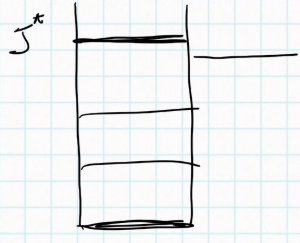
\includegraphics[scale=0.9]{Immagini/0325_lv.png}
    \caption{Livelli energetici del $\ce{^{20}Ne}$; la linea all'esterno rappresenta la reazione $p+\ce{^{19}F}$}
    \label{0325_lv}
\end{figure}
\noindent Come per l'elettrone, anche il nucleo presenta dei livelli energetici; se prendiamo per esempio la reazione $p+\ce{^{19}F}\to\ce{^{20}Ne}$, possiamo osservare dal disegno in Figura \ref{0325_lv} che la reazione è molto vicina al $\ce{^{20}Ne}^*$ per cui:
$$p+\ce{^{19}F}\to\ce{^{20}Ne}^*\to \ce{^{16}O} + \alpha$$
Si tratta quindi di una reazione $a+X$ che produce $Y+b$ passando per uno stadio intermedio $Z^*$ detto \textit{compound nucleus}\index{compound nucleus@\textit{compound nucleus}}; questo tipo di processo viene denominato \textbf{processo risonante}\index{processo risonante}\footnote{Si osservi che la $\sigma$ di tale processo è diversa sia da quella della reazione $a+X\to Y+b$ sia da $a+X\to Z$.}.

\subsubsection{Analisi Semi-classica}
Iniziamo studiando il processo con un approccio semi-classico. Se definiamo con $b$ il parametro di impatto per il proiettile $a$ sul bersaglio $X$, abbiamo per la sezione d'urto (classica) $\sigma = \pi b^2$; tale parametro in meccanica quantistica è legato alla quantità di moto da $b = \ell \: \hbar/p\equiv \ell\,\lambdabar_{DB}$\footnote{Abbiamo definito $\lambdabar_{DB}\equiv \lambda_{DB}/2\pi = \hbar/p$.}. Supponiamo di poter trascurare gli spin ($\ell$ si conserva) e dividere la zona di interazione in \vir{fette} al variare del valore di $\ell$: $0\leq \ell \leq 1$ allora $\sigma = \pi\lambdabar^2_{DB}$, $1\leq \ell \leq 2$ allora $\sigma = 3\pi\lambdabar^2_{DB}$ (area della corona); per un generico $\ell$
$$\sigma = \pi [(\ell+1)\lambdabar_{DB}]^2 - \pi[\ell\lambdabar_{DB}]^2 = (2\ell +1) \pi\lambdabar^2_{DB}$$
Dalla conservazione, $\ell$ è lo stesso per $Z^*$, quindi $\sigma(\ell)$ è la sezione d'urto d'eccitazione di $Z$.\\
Se a questo punto consideriamo anche gli spin ($J_a$, $J_X$,$\ell\to J$), sarà necessario eseguire una media per cui:
$$\sigma = \pi\lambdabar_{DB}\,\frac{2J+1}{(2J_a+1)(2J_X+1)}\equiv \pi\lambdabar_{DB}^2\,g$$
Inoltre ogni livello ha un certo allargamento di riga distribuito come una Lorentziana $f(E)$\footnote{$$f(E)=\frac{\Gamma^2}{(E-E_R)^2+(\Gamma/2)^2}$$} di cui tenere conto nell'espressione di $\sigma$.\\
Per quanto riguarda $Z^*$, abbiamo la possibilità sia che decada in $b+Y$ sia che faccia scattering elastico $a+X$, per cui ci sarà una certa probabilità di decadimento nell'$i$-esimo canale $P_i = \Gamma_i/\Gamma$, dove $\Gamma=\hbar/\tau$\footnote{$\tau$ tempo di decadimento.}; questa entra nella sezione d'urto per cui $\sigma\propto \Gamma_a\Gamma_b/\Gamma^2$. Si ottiene infine un'espressione per $\sigma$ detta \textbf{formula di \BW}\index{formula di \BW}\footnote{Abbiamo usato $p^2 = 2\mu E$.}:
$$\sigma = \pi\frac{\hbar^2}{2\mu E}g\Gamma_a\Gamma_b \frac{1}{(E-E_R)^2+(\Gamma/2)^2}$$

\subsubsection{Analisi Quantistica}
\begin{figure}[h]
    \centering
    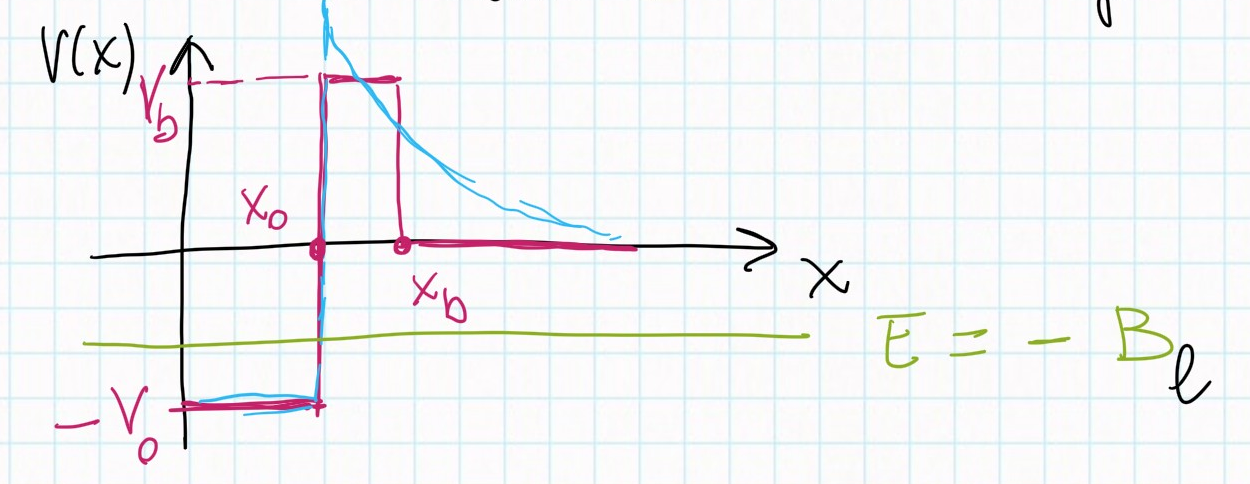
\includegraphics[scale=0.2]{Immagini/0325_pot.png}
    \caption{Schema della barriera di potenziale.}
    \label{0325_pot}
\end{figure}
\noindent Studiamo a questo punto il processo con l'approccio della meccanica quantistica\footnote{\label{0325_art}Si segue il calcolo riportato nell'articolo Charity, R.J., Eur. Phys. J. Plus, 2016, vol.131, art.63, \texttt{DOI:} \doi{10.1140/epjp/i2016-16063-1}.\articolo{Charity}}, servendoci però di un semplice \vir{modellino} unidimensionale a singola particella (come nel modello \textit{a shell}\index{modelli nucleari! a shell@\textit{a shell}} i nucleoni si muovono in un potenziale medio comune per tutti) dove non facciamo distinzione tra protoni e neutroni e rappresentiamo la barriera di potenziale come un \vir{muro} (Figura \ref{0325_pot}). Studiamo l'equazione di \Sch{} e le relative soluzioni per le varie zone ($x\lessgtr x_0,x_b$) per lo stato legato $E=-B_\ell$:
\begin{displaymath}
\begin{aligned}
\text{Equazioni}& & & \\
&1. & &-\frac{\hbar^2}{2m} \frac{d^2}{dx^2} \psi(x) = E\psi(x) & &x>x_b \\
&2. & &\ppc{-\frac{\hbar^2}{2m} \frac{d^2}{dx^2} + V_b} \psi(x) = E\psi(x) & &x_0<x<x_b \\
&3. & &\ppc{-\frac{\hbar^2}{2m} \frac{d^2}{dx^2}-V_0} \psi(x) = E\psi(x) & &x<x_0 \\
\text{Soluzioni}& & & \\
&1. & &\psi(x) = G\,e^{-k_\infty x} + \cancel{F\,e^{k_\infty x}} & &x>x_b \\
&2. & &\psi(x) = C\,e^{k_b x} + D\, e^{-k_b x} & &x_0<x<x_b \\
&3. & &\psi(x) = A\,\sin{(k_0x)} + \cancel{B\,\cos{(k_0x)}} & &x<x_0 
\end{aligned}
\end{displaymath}
$$k_0 \equiv \frac{\sqrt{2m(V_0-B_\ell)}}{\hbar}\qquad\quad k_b\equiv\frac{\sqrt{2m(V_b+B_\ell)}}{\hbar}\qquad\quad k_\infty\equiv\frac{\sqrt{2mB_\ell}}{\hbar}$$
Per trovare i vari coefficienti e $B_\ell$ si impone la continuità della funzione e della derivata prima e la normalizzazione. In Figura \ref{0325_ris} abbiamo riportato i risultati per $A=5$ nel fondamentale. 
\begin{figure}[!hb]
    \centering
    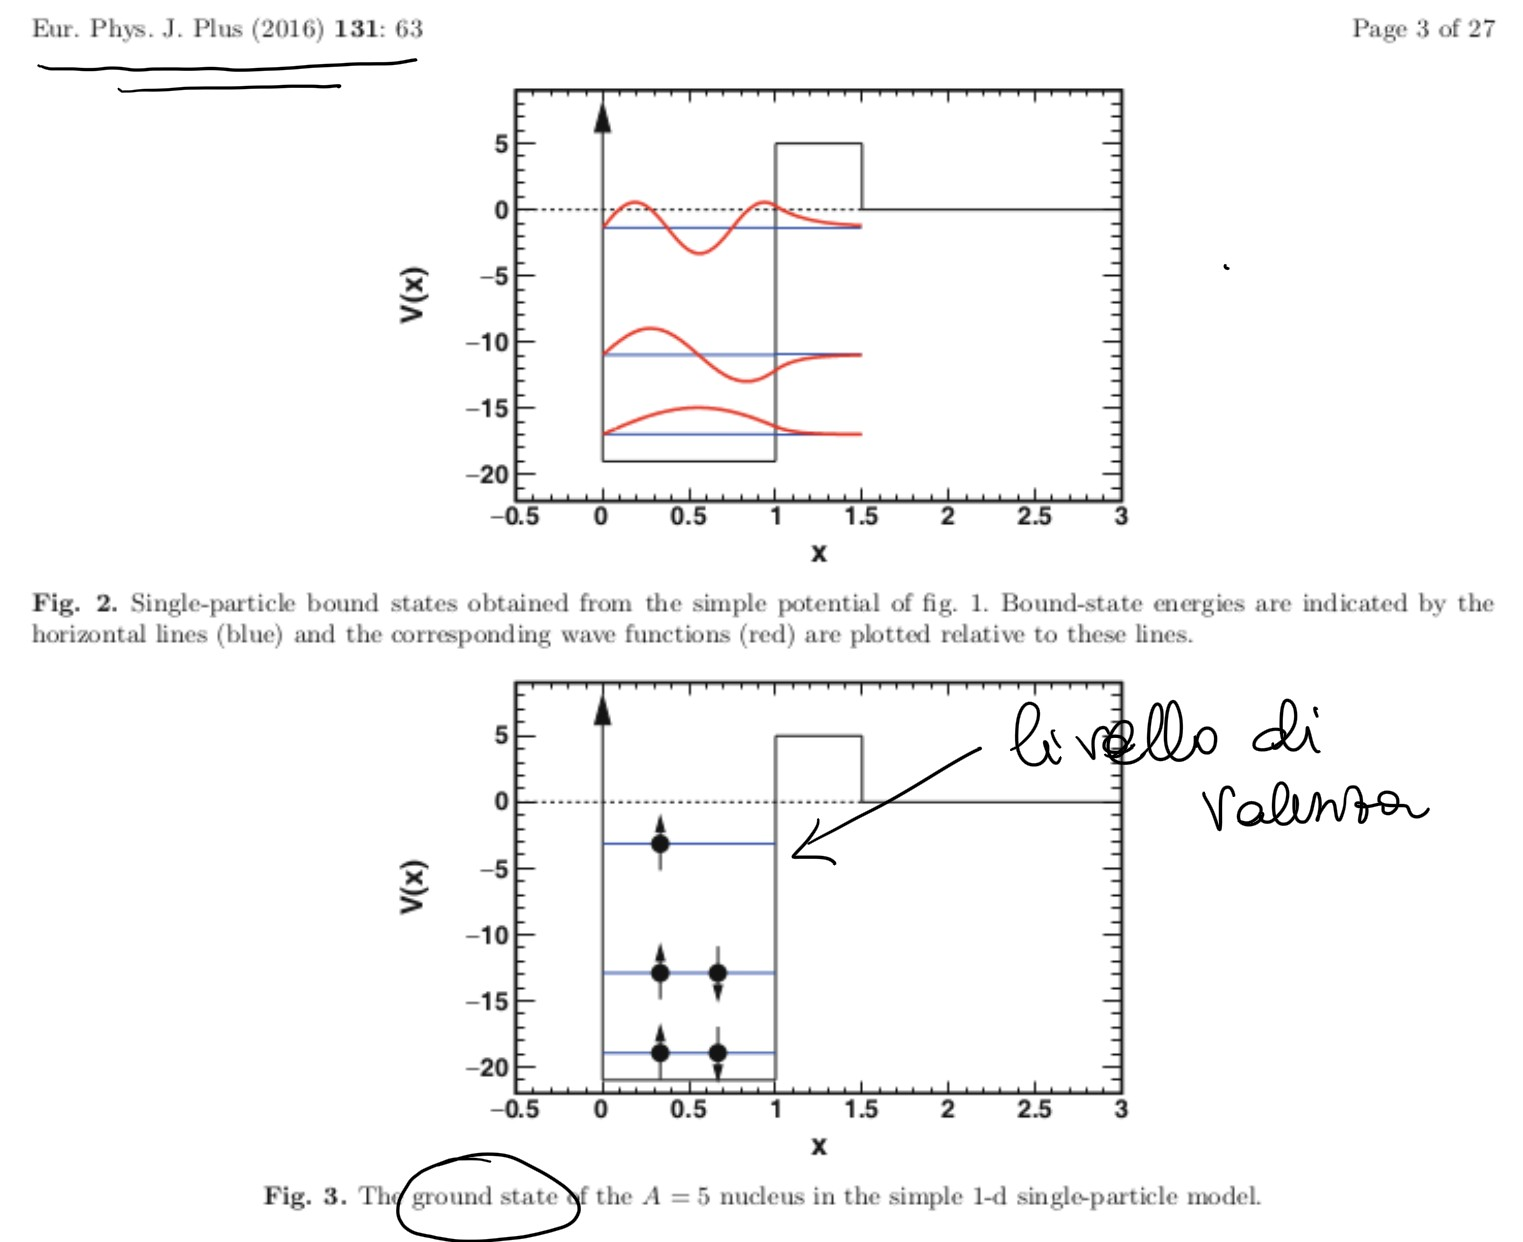
\includegraphics[scale=0.3]{Immagini/0325_risonanza.png}
    \caption{Grafici del potenziale e delle soluzioni del calcolo riportato nell'articolo.}
    \label{0325_ris}
\end{figure}
\noindent Come si ottiene lo stato eccitato? Si potrebbe promuovere un nucleone dal secondo livello a quello di valenza\index{livello di valenza}, ma questo non sarebbe lo stato risonante. Osserviamo però che modificando $V_0$ (cioè \vir{alzandolo}) si potrebbe fare in modo che l'energia del livello di valenza\index{livello di valenza} divenga positiva, ma rimanga inferiore a $V_b$ (Figura \ref{0325_potris}); esiterebbe allora una certa probabilità di \textit{tunneling}\footnote{$P_{tunnel} = 1 - P_{stay}$.} per quel nucleone:
$$\frac{dP_{stay}}{dt} = -\Gamma \, P_{stay} \quad \Rightarrow \quad P_{stay}\propto e^{-\Gamma t}$$
\begin{figure}[h]
    \centering
    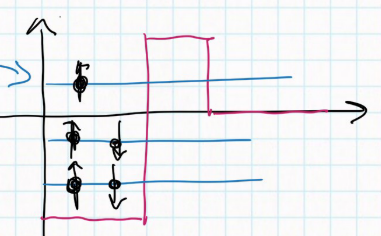
\includegraphics{Immagini/0325_po_risonanza.png}
    \caption{Schema dello stato risonante.}
    \label{0325_potris}
\end{figure}
\noindent Dobbiamo allora considerare l'equazione di \Sch{} in funzione del tempo\footnote{$$i\hbar \frac{d\psi}{dt}(x,t) = \ppc{-\frac{\hbar^2}{2m}\frac{d^2}{dx}+V}\psi(x,t)$$} e cercare una soluzione del tipo $\psi(x,t) = \exp{(-i t \, E/\hbar)}\,\psi(x)$, dove $\psi(x)$ è soluzione dell'equazione di \Sch{} precedente. Ora l'andamento di $P_{stay}$ impone\footnote{$P_{stay}\propto |\psi(x,t)|^2 = |\exp{(-i t \, E/\hbar)}|^2\,|\psi(x)|^2$} che $E\in \C$, per cui scegliamo $E = E_R - i \Gamma/2 \:\Rightarrow\: |\psi(x,t)|^2 = \exp{(-t\Gamma/\hbar)}\,|\psi(x)|^2$. Osserviamo che il termine di dipendenza temporale si fa sentire solo per $x>x_b$ (Figura \ref{0325_ris2}), dunque:
$$x>x_b \qquad \psi(x,t) = H\,e^{i\,(-\frac{E}{\hbar}\,t + i\,k_\infty x)}$$
\begin{figure}[h]
    \centering
    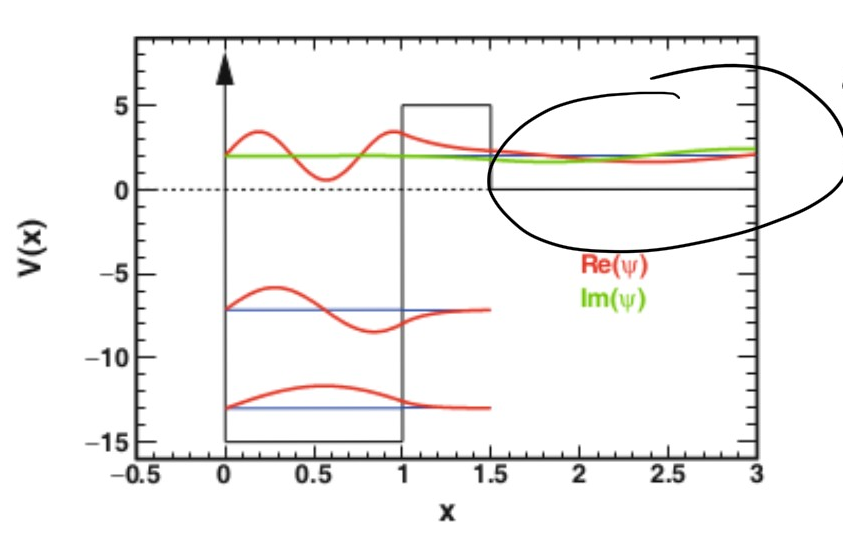
\includegraphics[scale=0.4]{Immagini/0325_risonanza2.png}
    \caption{Grafici del potenziale e delle soluzioni del calcolo riportato nell'articolo.}
    \label{0325_ris2}
\end{figure}
\noindent Questo non è quindi uno stato eccitato, ma una \textbf{risonanza}\index{processo risonante}\index{risonanza}. Dal punto di vista dello scattering, siamo interessati al processo inverso, ovvero all'effetto \textit{tunnel}\index{effetto tunnel} per entrare; dall'equazione di \Sch{}:
\begin{displaymath}
\begin{aligned}
\psi(x)&= A\, \sin{(k_\infty x +\delta)} = & &x>x_b \\
&= \frac{A}{2i} \, e^{-i\delta}\ppc{e^{i\,(k_\infty x + 2\delta)} - e^{-i\,k_\infty x}} & \\
\psi(x)&= C\, e^{k_b x} + D\, e^{-k_b x} & &x_0<x<x_b \\
\psi(x)&= A'\, \sin{(k_0 x)} & &x<x_0 
\end{aligned}
\end{displaymath}
La probabilità di penetrazione sarà data da $P_{in}\propto \int_0^{x_0} |\psi(x)|^2 dx$ e ne osserviamo i risultati in Figura \ref{0325_ris3}.
\begin{figure}[h]
    \centering
    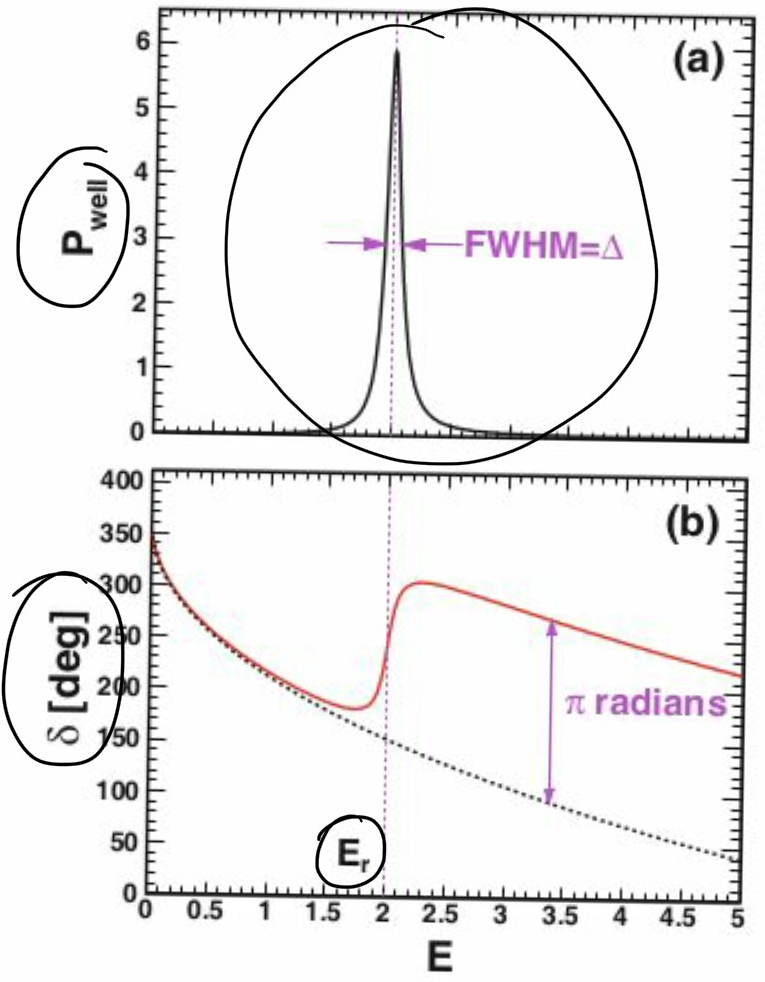
\includegraphics[scale=0.4]{Immagini/0325_risonanza3.png}
    \caption{Andamenti della probabilità di penetrazione e dello sfasamento in funzione dell'energia.}
    \label{0325_ris3}
\end{figure}
\noindent Si noti che l'andamento di $P_{in}\propto \Gamma^2/((E-E_r)^2+\Gamma^2/4)$ con $E_r$ energia del picco e $\Gamma = \,$FWHM e in particolar modo che per $E=E_r$ $\delta$ ha un salto di $\pi$ (questo è uno degli indicatori della presenza di una risonanza). Si ritrova allora la \BW\index{formula di \BW}.

\newpage

\subsubsection{Reaction-rate e fattore astrofisico}
Sostituiamo allora in $\mean{\sigma v}$ l'espressione di \BW{} per $\sigma$\footnote{Attenzione nelle note del corso vi è un errore: è riportato un $-$ al denominatore, invece di un $+$.}:
\begin{displaymath}
\begin{aligned}
\mean{\sigma v} &= \sqrt{\frac{8}{\pi\mu}} \ppc{\frac{1}{kT}}^{3/2} \frac{\pi\hbar^2}{2\mu} g \Gamma_a\Gamma_b \int_0^\infty \frac{1}{(E-E_R)^2 + (\Gamma/2)^2} \, e^{-E/kT} dE \simeq \\
&\simeq \sqrt{2\pi}\ppc{\frac{1}{\mu kT}}^{3/2} g\hbar^2 \Gamma_a\Gamma_b\, e^{-E_R/kT} \int_0^\infty \frac{dE}{(E-E_R)^2 + (\Gamma/2)^2} =\\
&= \sqrt{2\pi}\ppc{\frac{1}{\mu kT}}^{3/2} g\hbar^2 \Gamma_a\Gamma_b\, e^{-E_R/kT} \,\frac{2}{\Gamma} \arctan{(\frac{2}{\Gamma}(E-E_R))}\Bigr |_{0}^\infty \simeq \qquad \frac{E_R}{\Gamma}\to \infty \\
&\simeq \sqrt{2\pi}\ppc{\frac{1}{\mu kT}}^{3/2} g\hbar^2 \Gamma_a\Gamma_b\, e^{-E_R/kT} \, \frac{2\pi}{\Gamma} = \\
&= \ppc{\frac{2\pi}{\mu kT}}^{3/2} \hbar^2 \ppc{g\frac{\Gamma_a\Gamma_b}{\Gamma}}e^{-E_R/kT}
\end{aligned}
\end{displaymath}
dove abbiamo approssimato $\exp{(-E/kT)}\sim \exp{(-E_R/kT)}$, perché $E_R\gg \Gamma \sim 1$ eV e la distribuzione è molto piccata intorno $E_R$. Studiamo anche il fattore astrofisico\index{fattore astrofisico@fattore astrofisico $S(E)$}:
$$S(E)=E\, \sigma(E) \, e^{2\pi\frac{Z_1Z_2e^2}{\hbar v}}= \frac{\pi}{2\mu} \hbar^2 g \frac{\Gamma_a\Gamma_b}{(E-E_R)^2+(\Gamma/2)^2}e^{b/\sqrt{E}}$$
Prendiamo a titolo di esempio la reazione $p+\ce{^7Be}\to \ce{^8B} +\gamma$: $E_R=700$ keV, $\Gamma_p \simeq 35$ keV, $\Gamma_\gamma \simeq 25$ meV (trascurabile, $\Gamma \sim \Gamma_p$) e $b=0.99\cdot 3\,\sqrt{7/8}\unit{MeV}^{1/2}$. 

\paragraph{Tipologie di risonanze} Le risonanze si dividono principalmente in due tipologie in base al rapporto $\Gamma/E_R$:
\begin{itemize}
    \item \textbf{strette}\index{risonanza!stretta} $\Gamma/E_R<10\%$.
    \item \textbf{larghe}\index{risonanza!larga} $\Gamma/E_R>10\%$.
\end{itemize}
Il tipo di risonanza può essere significativo nello studio del fattore astrofisico\index{fattore astrofisico@fattore astrofisico $S(E)$}: se infatti la risonanza è stretta, nel caso in cui il \textit{range} di interesse sia lontano dal valore di risonanza le misure non risentono di alcun effetto del picco; al contrario con una risonanza larga, si possono avere effetti dovuti alle code della risonanza che alterano le acquisizioni (per esempio si registrano valori maggiori di quelli attesi senza la risonanza).

\subsubsection{Risonanze sotto soglia}
\begin{figure}[h]
    \centering
    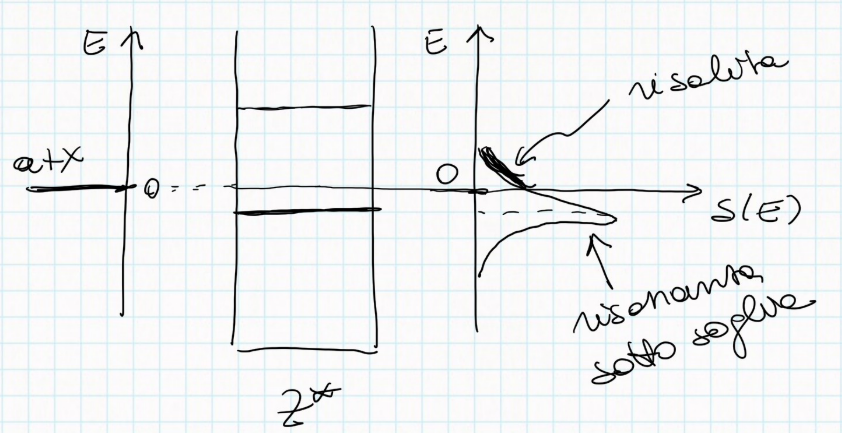
\includegraphics[scale=0.8]{Immagini/0325_risonanza4.1.png}
    \caption{Schema risonanza sotto soglia}
    \label{0325_ris41}
\end{figure}
\noindent Esiste anche un particolare tipo di risonanza detta \textbf{risonanza sotto soglia}\index{risonanza!sotto soglia}, per cui tra i livelli del \textit{compound nucleus}\index{compound nucleus@\textit{compound nucleus}} compare uno stato risonante sotto alla soglia della reazione (Figura \ref{0325_ris41}); se la risonananza è sufficientemente larga può influenzare le misure portando per esempio a un piccolo andamento crescente (\vir{una risalita}) del fattore astrofisico\index{fattore astrofisico@fattore astrofisico $S(E)$} per energie prossime a $E=0$ (Figura \ref{0325_ris4}). Questo dimostra l'importanza di una buona guida teorica nella zona di estrapolazione.

\begin{figure}[h]
    \centering
    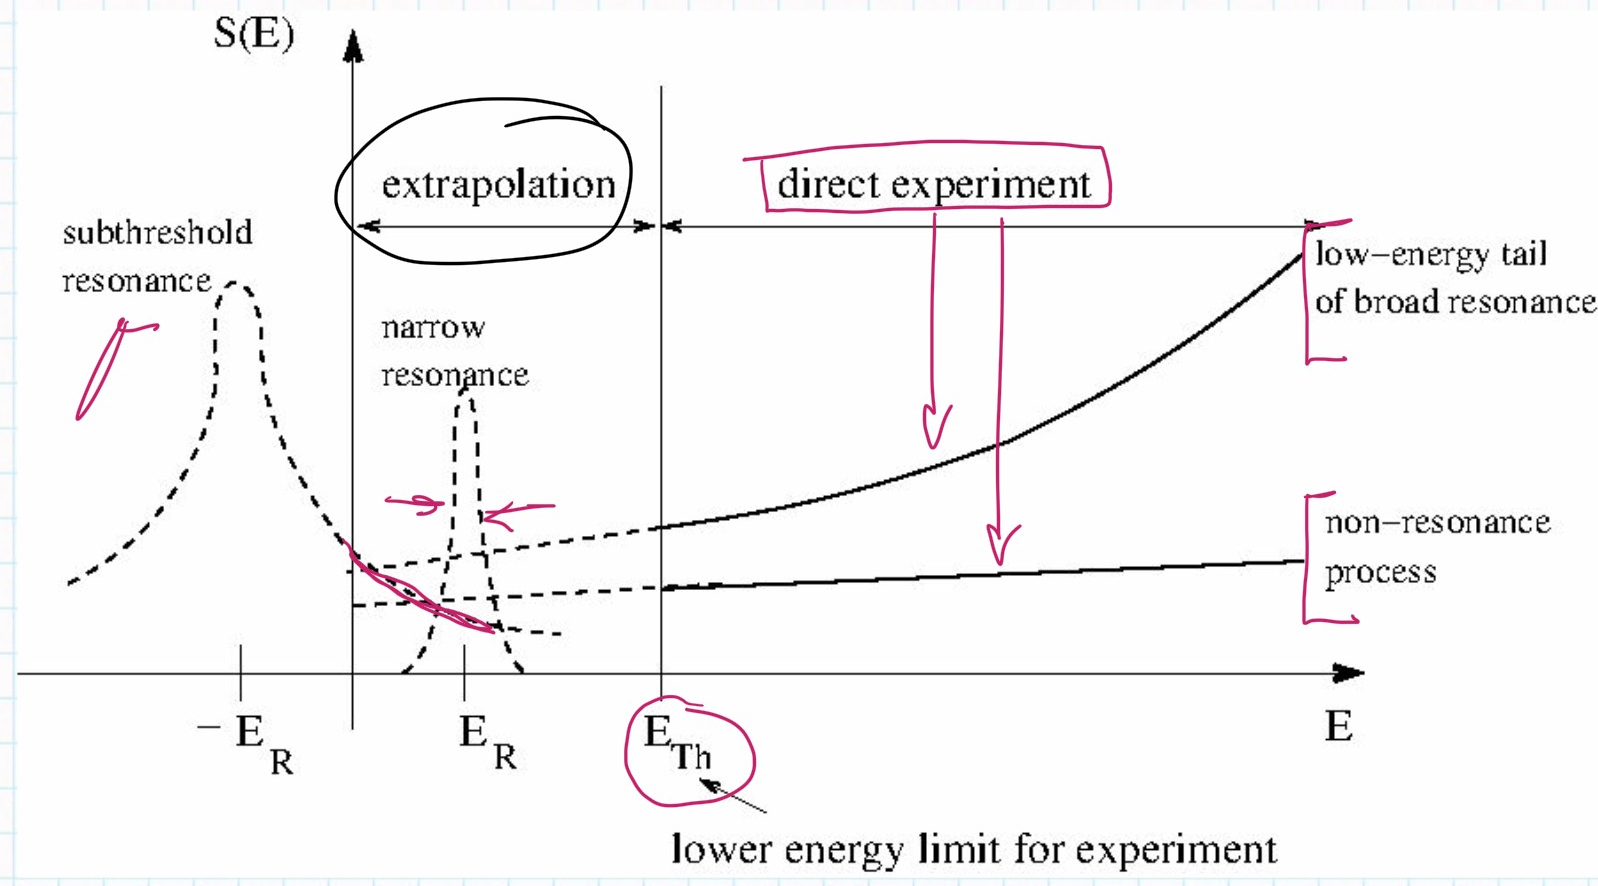
\includegraphics[scale=0.3]{Immagini/0325_risonanza4.png}
    \caption{Simulazione di una situazione sperimentale con risonanza sotto soglia. $E_{Th}$ è la minima energia raggiunta dagli esperimenti diretti.}
    \label{0325_ris4}
\end{figure}
\newpage
\subsubsection{Risonanza e neutrini solari}\label{0325-sec-risnu}
Abbiamo già studiato nella sezione \secrif{0322-sec-nu} come la questione dei neutrini solari, prima degli esperimenti di rivelazione delle oscillazioni di sapore, fosse un problema alquanto discusso\complementi{l'ipotesi di Fowler}. Tra le varie teorie avanzate ve ne fu una anche da parte di Fowler che prevedeva appunto la possibilità di una risonanza non studiata: egli supponeva che il calcolo del fattore astrofisico fosse sbagliato a causa di una risonanza o sotto soglia\index{risonanza!sotto soglia} o molto stretta\index{risonanza!stretta} nella reazione $\ce{^3He}+\ce{^3He}$ ($ppI$) nel \textit{range} di energie di interesse astrofisico (che nel 1980 non era ancora stato esplorato); dunque il valore di $S(E)$ sarebbe stato sottostimato. Tale soluzione, però, fu confutata dalle misure di LUNA\esperimento{LUNA}\footnote{Guarda \secrif{sec-LUNA-I}.} che dimostrarono l'assenza di qualsiasi tipo di risonanza.